\section{Representation of data}
%%%%%%%%%%%%%%%%%%%%%%%%%%%%%%%%%%%%%%%%%%%%%
%%%%%%%%%%%%%%%%%%%%%%%%%%%%%%%%%%%%%%%%%%%%%
%%%%%%%%%%%%%%%%%%%%%%%%%%%%%%%%%%%%%%%%%%%%%
%%%%%%%%%%%%%%%%%%%%%%%%%%%%%%%%%%%%%%%%%%%%%
%% 1.1 Terminologies %%%
%%%%%%%%%%%%%%%%%%%%%%%%%%%%%%%%%%%%%%%%%%%%%
%%%%%%%%%%%%%%%%%%%%%%%%%%%%%%%%%%%%%%%%%%%%%
%%%%%%%%%%%%%%%%%%%%%%%%%%%%%%%%%%%%%%%%%%%%%
%%%%%%%%%%%%%%%%%%%%%%%%%%%%%%%%%%%%%%%%%%%%%
\subsection{Terminologies}

Note the following terms:

\begin{itemize}

	\item qualitative data
	
	
	$\underline{\hspace{3cm}}$ or $\underline{\hspace{3cm}}$  are often used to show the information.
	\item quantitative data (numerical values)
	
	There are two types:  $\underline{\hspace{3cm}}$ and $\underline{\hspace{3cm}}$.
	
	
	\item frequency distribution
	
	Case $1$:
	\vspace{1cm}
	
	Case $2$:
	
	
	\item class boundry, interval width
	
\end{itemize}






\exercise  %% Exercise 1

\begin{enumerate}  %%% P1 example 1.1
	\item  The table shows the areas of different categories of land use in a particular region.
	\medskip
	
	\renewcommand{\arraystretch}{1.2} % default is 1.0
	\begin{tabular}{|c|c|c|c|c|c|}
		\hline
		Category &  Urban & Woodland & Farmland & Reservoris & Total \\ 
		\hline
		Area($\si{\km\squared}$) & 615 & 660 & 1200 & 225 & 2700 \\ 
		\hline
	\end{tabular}

\smallskip

Illustrate the data diagramatically.

\item  In a survey on the number of letters in the solutions of a crossword puzzle, the following data were obtained from the crossword puzzle in Monday's newspapaer.

\begin{tabular}{cccccccccc}
	\rule[-1ex]{0pt}{2.5ex} 9 & 5 & 7 & 7 & 5 & 12 & 6 & 6 & 12 & 5 \\
	\rule[-1ex]{0pt}{2.5ex} 7 & 7 & 5 & 5 & 3 & 7 & 3 & 7 & 9 & 6 \\
	\rule[-1ex]{0pt}{2.5ex} 3 & 5 & 7 & 3 & 6 & 7 & 7 & 6 & 3 & 7 \\
\end{tabular}

Draw a frequency distribution table for the data.



\item  The following data were obtained in a survey of heights of 20 children in a sports club. Each height was measured to the nearest centimetre.

\begin{tabular}{cccccccccc}
	\rule[-1ex]{0pt}{2.5ex} 133 & 136 & 120 & 138 & 133 & 131 & 127 & 141 & 127 & 143 \\
	\rule[-1ex]{0pt}{2.5ex} 130 & 131 & 125 & 144 & 128 & 134 & 135 & 137 & 133 & 129 \\
\end{tabular}

Draw a frequency distribution table for the data.
\end{enumerate}


\newpage


%%%%%%%%%%%%%%%%%%%%%%%%%%%%%%%%%%%%%%%%%%%%%
%%%%%%%%%%%%%%%%%%%%%%%%%%%%%%%%%%%%%%%%%%%%%
%%%%%%%%%%%%%%%%%%%%%%%%%%%%%%%%%%%%%%%%%%%%%
%%%%%%%%%%%%%%%%%%%%%%%%%%%%%%%%%%%%%%%%%%%%%
%% 1.2 Stem and leaf diagram %%%
%%%%%%%%%%%%%%%%%%%%%%%%%%%%%%%%%%%%%%%%%%%%%
%%%%%%%%%%%%%%%%%%%%%%%%%%%%%%%%%%%%%%%%%%%%%
%%%%%%%%%%%%%%%%%%%%%%%%%%%%%%%%%%%%%%%%%%%%%
%%%%%%%%%%%%%%%%%%%%%%%%%%%%%%%%%%%%%%%%%%%%%
\subsection{Stem-and-leaf diagram}

A way of grouping data into intervals while still retaining  the original data is to draw a \textbf{stem-and-leaf diagram}. 

\vspace{5 pt}


For example, there are 20 students in an assignment, their marks are as follows:
\vspace{5 pt}

\begin{tabular}{cccccccccc}
	\rule[-1ex]{0pt}{2.5ex} 84 & 17 & 38 & 45 & 47 & 53 & 76 & 54 & 75 & 32 \\
	\rule[-1ex]{0pt}{2.5ex} 66 & 65 & 55 & 54 & 51 & 44 & 39 & 19 & 54 & 72 \\
\end{tabular}

\vspace{5 pt}
A final plot of stem-and-leaf diagram would be like: 

\begin{table}[htbp]
	\centering
	

	
	\begin{tabular}{c|l@{\hspace{4 pt}}l@{\hspace{4 pt}}l@{\hspace{4 pt}}l@{\hspace{4 pt}}l@{\hspace{4 pt}}l@{\hspace{4 pt}} 	c}
		
		Stem & Leaf  & \\ 
		1     & 7 9 & (2)\\    
		2     &  & (0)\\    
		3     & 2 8 9 & (3)\\    
		4     & 4 5 7 & (3)\\    
		5     & 1 3 4 4 4 5 & (6)\\    
		6     & 5 6 & (2)\\
		7     & 2 5 6 & (3)\\
		8     & 4 &(1) \\
		
		
	\end{tabular}
\vspace{4 pt}

\fbox{ Key: $1 | 1 $ means 17 marks}

     \caption{Stem-and-leaf diagram of assignment marks}
	\label{tab:addlabel}
	
\end{table}

\textbf{Important}: You must always give a $\underline{\hspace{2 cm}}$ to explain what the stem and leaf  represent.
\medskip

 Also, $\underline{\hspace{4 cm}}$ must be chosen in a stem-and-leaf diagram.

\bigskip

For two sets of data, $\underline{\hspace{6 cm}}$ is often used to compare the data.


\exercise %% Exercise 2

\begin{enumerate} %% 
	\item  The lengths, in metres, of 20 measurements in a physics experiments are recorded as follows.
	\vspace{5 pt}
	
	\begin{tabular}{cccccccccc}
		\rule[-1ex]{0pt}{2.5ex} 1.78 & 1.87 & 1.89 & 1.72 & 1.68 & 2.04 & 1.96 & 1.76 & 1.90 & 1.73 \\
		\rule[-1ex]{0pt}{2.5ex} 1.78 & 1.61 & 1.78 & 1.77 & 1.85 & 1.65 & 1.89 & 1.95 & 2.01 & 1.83 \\
	\end{tabular}
\begin{enumerate}
	\item Represent this information on a stem-and-leaf diagram.
	\item State the mode.
\end{enumerate}
 


\item The maximum temperature in $\si{\celsius}$, measured to the nearest degree, was recorded each day during June in a particular city. The temperature were as follows:

\begin{tabular}{ccccccccccccccc}
	\rule[-1ex]{0pt}{2.5ex} 19 & 23 & 19 & 19 & 20 & 12 & 19 & 22 & 22 & 16 & 18 & 16 & 19 & 20 & 17 \\
	\rule[-1ex]{0pt}{2.5ex} 13 & 14 & 12 & 15 & 17 & 16 & 17 & 19 & 22 & 22 & 20 & 19 & 19 & 20 & 20 \\
\end{tabular}

Draw a stem-and-leaf diagram to illustrate the temperatures and write down the mode.


\item These are the examination marks for French and for English achieved by pupils in a particular class.

\begin{tabular}{ccccccccccc}
	\rule[-1ex]{0pt}{2.5ex} French & 43 & 55 & 29 & 49 & 36 & 55 & 61 & 34 & 42 & 42 \\
	\rule[-1ex]{0pt}{2.5ex}    & 54 & 60 & 48 & 23 & 44 & 31 & 55 & 45 & 37 & 57 \\
	\rule[-1ex]{0pt}{2.5ex} English & 80 & 65 & 74 & 59 & 79 & 92 & 52 & 71 & 43 & 86 \\
	\rule[-1ex]{0pt}{2.5ex}    & 60 & 74 & 57 & 41 & 79 & 74 & 58 & 52 & 64 & 84 \\
\end{tabular}

Draw a back-to-back stem-and-leaf diagram to compare the two sets of marks.
	
\end{enumerate}









%%%%%%%%%%%%%%%%%%%%%%%%%%%%%%%%%%%%%%%%%%%%%
%%%%%%%%%%%%%%%%%%%%%%%%%%%%%%%%%%%%%%%%%%%%%
%%%%%%%%%%%%%%%%%%%%%%%%%%%%%%%%%%%%%%%%%%%%%
%%%%%%%%%%%%%%%%%%%%%%%%%%%%%%%%%%%%%%%%%%%%%
%% 1.3 Histogram %%%
%%%%%%%%%%%%%%%%%%%%%%%%%%%%%%%%%%%%%%%%%%%%%
%%%%%%%%%%%%%%%%%%%%%%%%%%%%%%%%%%%%%%%%%%%%%
%%%%%%%%%%%%%%%%%%%%%%%%%%%%%%%%%%%%%%%%%%%%%
%%%%%%%%%%%%%%%%%%%%%%%%%%%%%%%%%%%%%%%%%%%%%

\newpage 

\subsection{Histograms}

Grouped data can be displayed in a \textbf{histogram}, as in the following diagram:
\vspace{0.5cm}

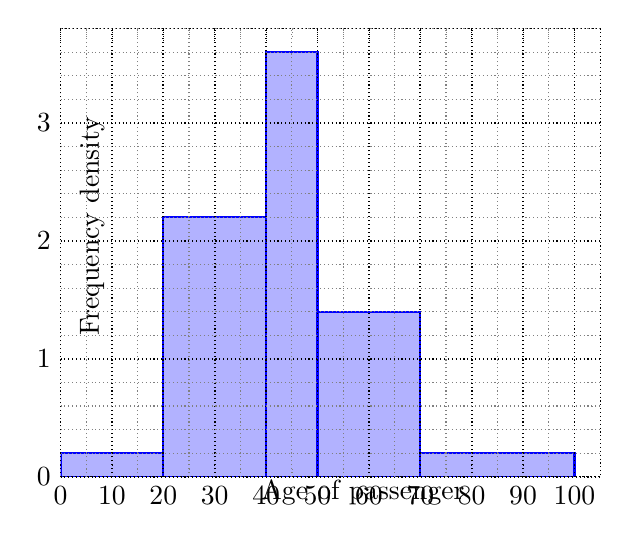
\begin{tikzpicture}
\centering

\begin{axis}[
area style,
densely dotted,
grid = both,
minor grid style=gray,
major grid style =black,
major grid style ={line width =0.6pt},
%	major grid style =thick,
major tick style=black,	
xmin = 0, xmax=105,
ymin=0, ymax= 3.8,
grid = both,
minor y tick num=4,
minor x tick num=1,
xtick={0,10,20,30,40,50,60,70,80,90,100},
xticklabels={0,10,20,30,40,50,60,70,80,90,100},	
x label style={at={(current axis.right of origin)},anchor=north, below=2mm, left =16mm},
y label style={at={(current axis.above origin)},anchor = west, below =4mm,left = 10mm},
xlabel={Age of passenger},
ylabel={Frequency density}
]


\addplot+[ybar interval,mark=no,thick,solid] plot coordinates { 
	(0,.2)
	(20,2.2)
	(40,3.6)
	(50,1.4)
	(70,0.2)
	(100,.2)
	
};


\end{axis}
\end{tikzpicture}

The frequency distribution table would be like:
\vspace{0.5cm}

\renewcommand{\arraystretch}{1.2} % default is 1.0
\begin{tabular}{|c|c|c|c|c|c|}
	\hline
	Age, $x$ years & $0 \leqslant x < 20$  & $20 \leqslant x < 40$ & $40 \leqslant x < 50$ & $50 \leqslant x < 70$ & $70 \leqslant x < 100$ \\
	\hline
	Frequency &  &  &  &  &  \\
	\hline
\end{tabular}

\bigskip

Notice the difference between histogram and $\underline{\hspace{2 cm}}$:

\begin{itemize}
	\setlength\itemsep{4em}
	\item 
	\item 
\end{itemize}

\bigskip

Frequency density:

\[
\text{frequency density} = \frac{\text{\qquad \qquad frequency \qquad \qquad  }}{}.
\]

\vspace{1cm}

Modal class: the interval with the greatest $\underline{\hspace{4 cm}}$.

\vspace{0.5cm}

Gaps treatment:

\begin{itemize}
	\setlength\itemsep{4em}
	\item Gropued continuous data (rounded values)
	\item Grouped discrete data (continuity correction, "0"): 
\end{itemize}
\vspace{0.5cm}





\newpage

The shape of a distribution:

\medskip
\vspace{6cm}

Positive skew  \hspace{4.2cm} Symmetrical  \hspace{4.2cm} \hfill Negative skew



 \exercise  %% Exercise 3

\begin{enumerate}
	\item A survey on the duration of telephone calls made to an office on a particular day gave the following results.
	
	\medskip
	
	%\renewcommand{\arraystretch}{1.2} % default is 1.0
	\begin{tabular}{|c|c|c|c|c|}
		\hline
		Duration, $t$ minutes & $1 \leqslant t < 3$  & $3 \leqslant t < 9$ & $9 \leqslant t < 15$ & $15 \leqslant t < 20$  \\
		\hline
		Frequency & 10 & 42 & 12 & 7   \\
		\hline
	\end{tabular}
\smallskip

     Draw a histogram to represent the data.
     
     \item The grouped frequency table records the weights, to the nearest gram, of the letters delievered to an apartment block on a particular day.
     
     	\medskip
     
     %\renewcommand{\arraystretch}{1.2} % default is 1.0
     \begin{tabular}{|c|c|c|c|c|c|}
     	\hline
     	Weight (gram) & $31-50$  & $51-60$ & $61-70$ & $71-100$ & $101-150$ \\
     	\hline
     	Frequency & 16 & 25 & 36 & 33 & 10   \\
     	\hline
     \end{tabular}
 \smallskip
 
 Draw a histogram to represent the data and state the modal class.
 
 \item $\dagger$ One evening a waiter measured the amounts of water left by diners in the bottles on the table in a restaurant. The volume were measured to the nearest millimetre.
 
 	\medskip
 
 %\renewcommand{\arraystretch}{1.2} % default is 1.0
 \begin{tabular}{|c|c|c|c|c|}
 	\hline
 	Volume (nearest \si{\ml}) & $0-19$  & $20-39$ & $40-89$ & $90-189$  \\
 	\hline
 	Frequency & 10 & 8 & 12 & 20   \\
 	\hline
 \end{tabular}
 \smallskip
 
  Draw a histogram to represent the data and state the modal class.
  
  \item These are marks in a statistics test for a group of 120 A level students.
  	\medskip
  
  %\renewcommand{\arraystretch}{1.2} % default is 1.0
  \begin{tabular}{|c|c|c|c|c|c|}
  	\hline
  	Mark & $0-9 $  & $10-19$ & $20-29$ & $30-49$ & $50-79$ \\
  	\hline
  	Frequency & 8 & 21 & 53 & 28 & 10   \\
  	\hline
  \end{tabular}
  \smallskip
  
  Draw a histogram to represent the data.
  \newpage 
  \item A Passenger's Association conducted a survey on the lateness of trains arriving at a particular railway station. The results are illustrated in the histogram.  
  \vspace{0.5cm}
  
  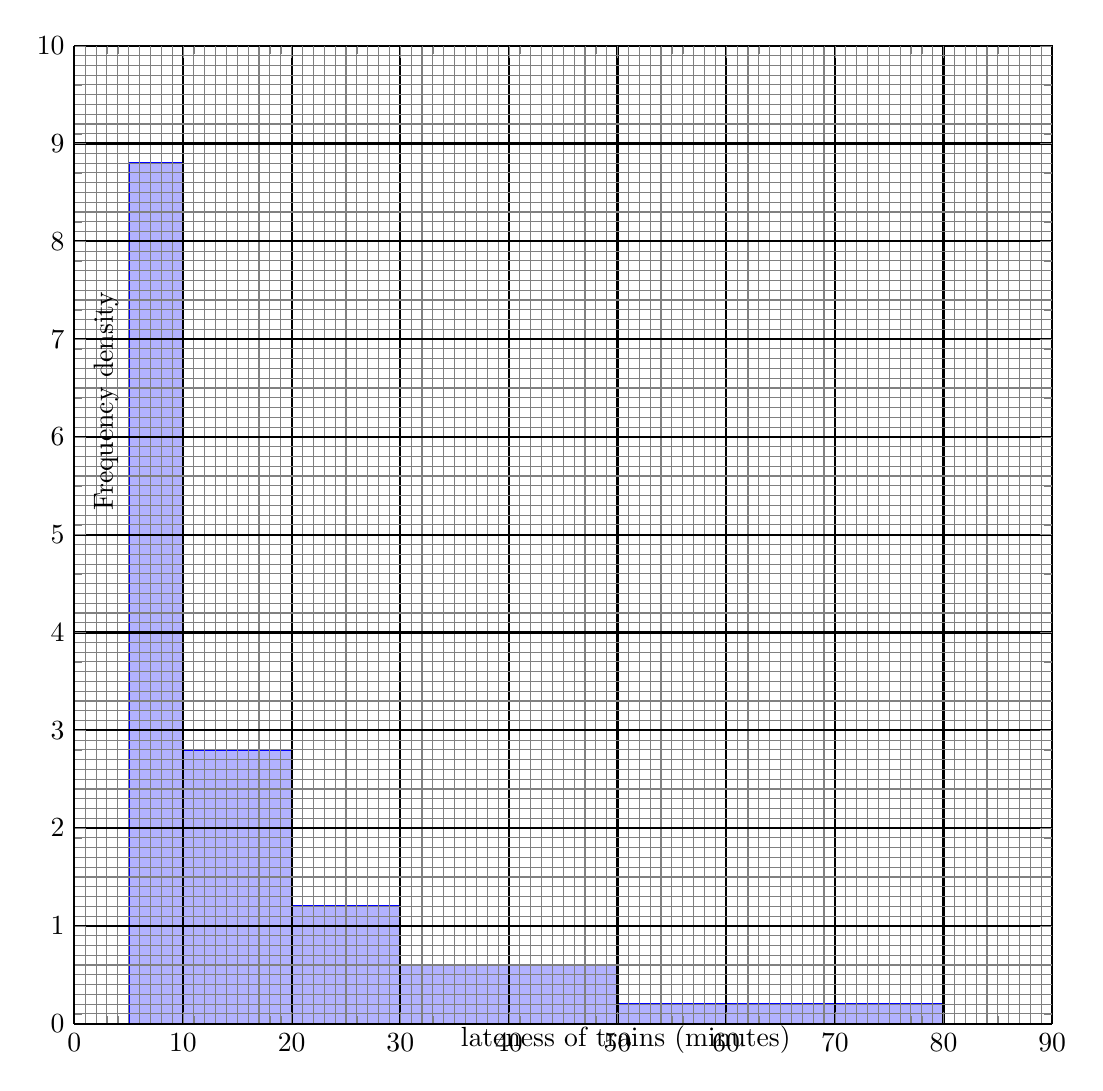
\begin{tikzpicture}
  \centering
  
  \begin{axis}[
  	width=14cm,
  	height=14cm,
  area style,
  solid,
  grid = both,
  minor grid style=gray,
  major grid style =black,
  major grid style ={line width =0.8pt},
  xmin = 0, xmax=90,
  ymin=0, ymax= 10,  
  minor y tick num=9,
  minor x tick num=9, 
  xtick={0,10,20,30,40,50,60,70,80,90},
  xticklabels={0,10,20,30,40,50,60,70,80,90},
  ytick={0,1,2,3,4,5,6,7,8,9,10},
  yticklabels={0,1,2,3,4,5,6,7,8,9,10}, 
  x label style={at={(current axis.right of origin)},anchor=north, below=2mm, left =32mm},
  y label style={at={(current axis.above origin)},anchor = west, below =4mm,left = 30mm},
  xlabel={lateness of trains (minutes)},
  ylabel={Frequency density}
  ]
  
  
  \addplot+[ybar interval,mark=no,thick,solid] plot coordinates { 
  	(0,6.4)
  	
  	(5,8.8)
  	(10,2.8)
  	(20,1.2)
  	(30,0.6)
  	(50,0.2)
  	(80,0)
  	
  };
  
  
  \end{axis}
  \end{tikzpicture}
  
  \begin{enumerate}
  	\item Construct a frequency table
  	\item What percentage of the train were less than 20 minutes late?
  \end{enumerate}
 
	
	
\end{enumerate}

\newpage

%%%%%%%%%%%%%%%%%%%%%%%%%%%%%%%%%%%%%%%%%%%%%
%%%%%%%%%%%%%%%%%%%%%%%%%%%%%%%%%%%%%%%%%%%%%
%%%%%%%%%%%%%%%%%%%%%%%%%%%%%%%%%%%%%%%%%%%%%
%%%%%%%%%%%%%%%%%%%%%%%%%%%%%%%%%%%%%%%%%%%%%
%% 1.4 Average %%%
%%%%%%%%%%%%%%%%%%%%%%%%%%%%%%%%%%%%%%%%%%%%%
%%%%%%%%%%%%%%%%%%%%%%%%%%%%%%%%%%%%%%%%%%%%%
%%%%%%%%%%%%%%%%%%%%%%%%%%%%%%%%%%%%%%%%%%%%%
%%%%%%%%%%%%%%%%%%%%%%%%%%%%%%%%%%%%%%%%%%%%%
\subsection{Average}

An \textbf{average} value is useful when describing a set of data. This is a typical or representative value and is known as a $\underline{\hspace{6 cm}}$.

\medskip

Mean: in general, the mean of the $n$ numbers $x_1,x_2,\cdots, x_n$ is given by
\[
\bar{x} = 
\]
Mean of a frequency distribution:
\begin{itemize}
	\item Discrete data
	\item Continuous data (\textbf{Mid-interval value})
	
	
	
\end{itemize}


\exercise  %% Exercise 4

\begin{enumerate}
	\item To obtain Grade $A$, Ben must achieve a mean mark of at least 70 in five test. His mean mark for the first four tests in 68, 	what is the lowest mark Ben could achieve in the fifth 	test to obtain Grade $A$.
	
	\item The numbers of an orchestra were asked how many instruments each could play. These are their replies.

	\begin{tabular}{ccccccccccccccc}
		\rule[-1ex]{0pt}{2.5ex} 2 & 5 & 2 & 4 & 1 & 1 & 1 & 2 & 1 & 3 & 3 & 2 & 1 & 2 & 1 \\
		\rule[-1ex]{0pt}{2.5ex} 1 & 2 & 4 & 3 & 2 & 1 & 2 & 3 & 1 & 4 & 2 & 3 & 1 & 1 & 2 \\
	\end{tabular}
	
\smallskip
	
	Calculate the mean number of instruments played.
	
	\item In a spot check, the speeds of 120 vehicles on a particular stretch of road through a village were noted. The results are shown in the table.
	\medskip

	
	%\renewcommand{\arraystretch}{1.2} % default is 1.0
	\begin{tabular}{|c|c|c|c|c|c|}
		\hline
		Speed $x$ \si{\km\per\hour} & $21-25 $  & $26-30$ & $31-35$ & $36-45$ & $46-60$ \\
		\hline
		Frequency $f$ & 22 & 48 & 25 & 16 & 9   \\
		\hline
	\end{tabular}
\medskip

	
	Estimate the mean speed of these vehicles.
	
	\item The diagram shows a histogram of distribution of the weights of 50 first-year students at a particular university. All the rectangles have been drawn, but the vertical scale is missing.

	
	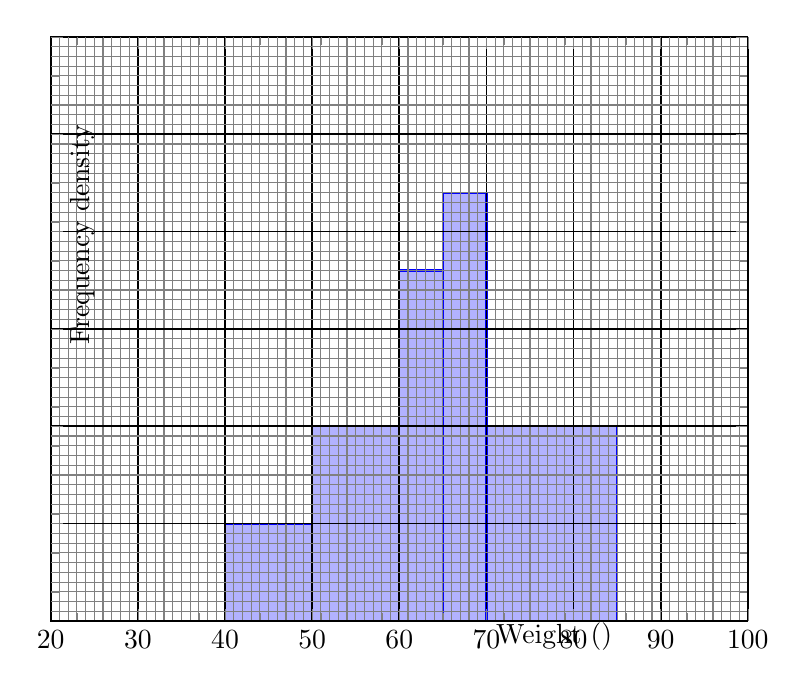
\begin{tikzpicture}
	\centering
	
	\begin{axis}[
	area style,
	height=9cm,
	solid,
	grid = both,
	minor grid style=gray,
	major grid style =black,
	major grid style ={line width =0.6pt},
	xmin = 20, xmax=100,
	ymin=0, ymax= 3,
	minor y tick num=9,
	minor x tick num=9, 
	xtick={20,30,40,50,60,70,80,90,100},
	xticklabels={20,30,40,50,60,70,80,90,100},
	ytick={0,0.5,1,1.5,2,2.5,3},
	yticklabels={\empty,\empty,\empty,\empty,\empty,\empty,\empty}, 	
	x label style={at={(current axis.right of origin)},anchor=north, below=2mm, left =16mm},
	y label style={at={(current axis.above origin)},anchor = west, below =4mm,left = 10mm},
	xlabel={Weight (\si{\kilogram})},
	ylabel={Frequency density}
	]	
	\addplot+[ybar interval,mark=no,thick,solid] plot coordinates { 
		(40,0.5)		
		(50,1)
		(60,1.8)
		(65,2.2)
		(70,1)
		(85,0)		
	};	
	\end{axis}
	\end{tikzpicture}
	
 Compile a grouped frequency table and find an estimate of the mean weight of these students.	

\end{enumerate}


\newpage

%%%%%%%%%%%%%%%%%%%%%%%%%%%%%%%%%%%%%%%%%%%%%
%%%%%%%%%%%%%%%%%%%%%%%%%%%%%%%%%%%%%%%%%%%%%
%%%%%%%%%%%%%%%%%%%%%%%%%%%%%%%%%%%%%%%%%%%%%
%%%%%%%%%%%%%%%%%%%%%%%%%%%%%%%%%%%%%%%%%%%%%
%% 1.5 Variation %%%
%%%%%%%%%%%%%%%%%%%%%%%%%%%%%%%%%%%%%%%%%%%%%
%%%%%%%%%%%%%%%%%%%%%%%%%%%%%%%%%%%%%%%%%%%%%
%%%%%%%%%%%%%%%%%%%%%%%%%%%%%%%%%%%%%%%%%%%%%
%%%%%%%%%%%%%%%%%%%%%%%%%%%%%%%%%%%%%%%%%%%%%
\subsection{Variability of data}


Range:


\vspace{1.5cm}

Variation:

\vspace{1.5cm}

Standard deviation:
\vspace{2cm}

Comparing distributions:  the $\underline{\hspace{3 cm}}$ the standard deviation, the $\underline{\hspace{3 cm}}$ there is and the $\underline{\hspace{3 cm}}$ the data are.
\medskip

'Calculation' version of formula for standard deviation: 

\[
\text{s.d.} = \sqrt{\frac{\sum x^2 }{n}  - \bar{x}^2},\quad \text{where} \quad \bar{x} = \frac{\sum x}{n}.
\] 

Standard deviation of a frequency distribution:

\begin{itemize}
	\item Case $1$
	\item Case $2$
\end{itemize}


\exercise  %%%  Exercise 5

\begin{enumerate}
	\item The mean of the numbers $2,3,5,6,8$ is $4.8$. Calculate the standard deviation.
	
	\item  The distribution shows the number of children in $20$ families. The mean number of children in a family is 2.9. Calculate  the range and the standard deviation.
	
		\medskip
	
	\renewcommand{\arraystretch}{1.2} % default is 1.0
	\begin{tabular}{|c|c|c|c|c|c|}
		\hline
		Number of children, $x$ & $ 1$ & $2$ & $3$ & $4$ & $5$ \\ 
		\hline
		Number of families, $f$ & $3$ & $4$ & $8$ & $2$ & $3$ \\ 
		\hline
	\end{tabular}
	
	\smallskip
	
	
	\item  An online test was taken by 115 students. The time spent on each question was recorded by the computer. The following table shows the time taken, in minutes, on the final question.
		\medskip
	
	\renewcommand{\arraystretch}{1.2} % default is 1.0
	\begin{tabular}{|c|c|c|c|c|}
		\hline
		Time (mins) &  $1\leq x <2$ & $2\leq x <3$ & $3\leq x <5$ & $5\leq x <10$  \\ 
		\hline
		Frequency & $16$ & $32$ & $42$ & $25$  \\ 
		\hline
	\end{tabular}
	
	\smallskip
	
	Calculate estimates of the mean and standard deviation of the time spent on the final question.
	
	\item Becky plays a computer game where she fires at a target. Her score is 1 if she hits the target and 0 if she misses it.
	
	She has 30 attempts and hits the target 18 times.
	
	\begin{enumerate}
		\item Find her mean score for the 30 attempts.
		\item Find the variance of her scores for the 30 attempts.
	\end{enumerate} 
	
	
\end{enumerate}


\newpage



\textbf{Combining sets of data}:
\smallskip

In general, for two sets of data, $x$ and $y$:
\[
\text{mean} = \frac{\sum x + \sum y}{n_1+n_2}, \qquad   \text{stand deviation} = \sqrt{\frac{\sum x^2 + \sum y^2}{n_1+n_2}- (\text{mean})^2}. 
\]


\textbf{Coding data}
\smallskip

In general, if each data value is increased by a constant $a$, 

\begin{itemize}
	\setlength\itemsep{0.8em}
	\item  the mean is  $\underline{\hspace{3cm}}$         .  That is 
	\[
	\bar{x} = \frac{\sum (x-a)}{n} +   a.
	\]
	\item   the standard deviation is $\underline{\hspace{2 cm}}$. That is 
	\[
	\text{s.d. of } x = \sqrt{\frac{\sum (x-a)^2}{n} -  \left(\frac{\sum (x-a)}{n}\right)^2}.  
	\]
\end{itemize}


\exercise   %%%  --- Exercise 6

\begin{enumerate}
	\item The ages, $x$ years, of $18$ people attending an evening class are summarized by the following totals:
	\[
	\sum x = 745,  \qquad \sum x^2 = 33951.
	\]
	\begin{enumerate}
		\item Calculate the mean and the standard deviation of the ages of this group of people.
		\item One person leaves the group and the mean age of the remaining $17$ people is exactly $41$ years. Find the age of the person who left and the standard deviation of the ages of the remaining $17$ people.
	\end{enumerate}
	
	
	\item The following table shows the mean and standard deviation of the heights of $20$ boys and $30$ girls.
	
	\medskip
	\begin{table}[!htpb]
		\centering

\begin{tabular}{|c|c|c|} 
	\cline{2-3}
	\multicolumn{1}{l|}{} & Mean   & Standard deviation  \\ 
	\hline
	Boys                  & $160$ \si{\cm}  & $4$ cm               \\ 
	\hline
	Girls~                & $155$ cm & $3.5$ cm              \\
	\hline
\end{tabular}
	\end{table}
Find the mean and standard deviation of the heights of the $50$ children.


\item  Sweets are packed into bags with a nominal weight of 75 grams. Ten bags are picked at random from the production line and weighted. Their weights, in gram, are 

\vspace{5 pt}

\begin{tabular}{cccccccccc}
	\rule[-1ex]{0pt}{2.5ex}  $76.0$ &$74.2$ & $75.1$ & $73.7$ & $72.0$ & $74.3$ & $75.4$ & $74.0$ & $73.1$ & $72.8$ \\

\end{tabular}

\smallskip

	\begin{enumerate}
		\item Use your calculator to find the mean and the standard deviation .
		\item It is later discovered that the scales were reading 3.2 grams below the correct weight.
		\begin{enumerate}
			\item What was the correct mean weight of the $10$ bags?
			\item What was the correct standard deviation of the $10$ bags?
		\end{enumerate}
	\end{enumerate}


\item The time taken, $x$ minutes, by Katy  to do the Sudoku puzzle in a certain newspaper was observed on $20$ occasions. The results are summarised below.
\[
\sum (x-30) = -50   \qquad \qquad \sum (x-30)^2 =562
\]
Find the mean and standard deviation of the time taken by Katy to solve the Sudoku puzzle.




\item  A summary of $24$ observations of $x$ gave the following informations:
\[
\sum (x-a) = -73.2   \qquad \qquad \sum (x-a)^2 =2115
\]
The mean of these values of $x$ is $8.95$.
\begin{enumerate}
	\item Find the value of the constant $a$.
	\item Find the standard deviation of these value of $x$.
\end{enumerate}



\item  Delip measured the speeds, $x$ \si{\km} per hour, of  $70$ cars on a road where the speed limit is $60$ \si{\km} per hour. His results are summarised by  $\displaystyle \sum (x-60) = 245$.

\begin{enumerate}
	\item Calculate the mean speed of these cars.
\end{enumerate}

His friend Sachim used values of $(x-50)$ to calculate the mean

\begin{enumerate}[resume]
	\item  Find $\displaystyle \sum (x-50)$.
	\item The standard deviation of the speeds is $10.6$ \si{\km} per hour. Calculate  $\displaystyle \sum (x-50)^2$.
\end{enumerate}


\item It is known that, for $100$ observations of $x$, the mean $\bar{x} = 25$.

Find 
\begin{enumerate}
	\item $\displaystyle \sum x$, \,\,\, $\displaystyle \sum (x-20)$,  \,\,\,$\displaystyle \sum (x-27)$.
\end{enumerate} 

Given also that the standard deviation of $x$ is $3$, find 

\begin{enumerate}[resume]
	\item $\displaystyle \sum x^2$,  \,\, \, $\displaystyle \sum (x-20)^2$,  \, \,\,$\displaystyle \sum (x-27)^2$.
\end{enumerate}





\end{enumerate}

\newpage

%%%%%%%%%%%%%%%%%%%%%%%%%%%%%%%%%%%%%%%%%%%%%
%%%%%%%%%%%%%%%%%%%%%%%%%%%%%%%%%%%%%%%%%%%%%
%%%%%%%%%%%%%%%%%%%%%%%%%%%%%%%%%%%%%%%%%%%%%
%%%%%%%%%%%%%%%%%%%%%%%%%%%%%%%%%%%%%%%%%%%%%
%% 1.6 Cumulative frequency graph %%%
%%%%%%%%%%%%%%%%%%%%%%%%%%%%%%%%%%%%%%%%%%%%%
%%%%%%%%%%%%%%%%%%%%%%%%%%%%%%%%%%%%%%%%%%%%%
%%%%%%%%%%%%%%%%%%%%%%%%%%%%%%%%%%%%%%%%%%%%%
%%%%%%%%%%%%%%%%%%%%%%%%%%%%%%%%%%%%%%%%%%%%%
\subsection{Cumulative frequency graph}
\smallskip

When a set of data contains extreme values, known as $\underline{\hspace{2 cm}}$, the median is a more informative average and the interquartile range is more-useful measure of spread. 

\medskip

\textbf{Median}: for a set of $n$ numbers arranged in $\underline{\hspace{4 cm}}$.

\begin{itemize}
		\setlength\itemsep{0.8em}
	\item When $n$ is odd, 
	\item  When $n$ is even,
\end{itemize}


\textbf{Quartiles}:

\begin{itemize}
	\setlength\itemsep{0.8em}
	\item Lower quartile, $Q_1$, 
	\item  Upper quartile, $Q_3$, 
	\item  Interquartile range (IQR), 
\end{itemize}
\bigskip


\textbf{Cumulative frequency}: a total frequency up to a particular item. It is particular useful when finding the median and quartiles. 

\medskip  

\begin{itemize}
	\setlength\itemsep{0.8em}
	\item Ungrouped data
	\item  grouped data,  class boundaries.
 
\end{itemize}
\bigskip

\exercise  %%%  -- Exercise 7

\begin{enumerate}
	\item Find the median 	of each of these sets of numbers:
	\begin{enumerate}
		\item $7,7,2,3,4,2,7,9,31$
		\item  $36,41,27, 32,29, 39, 39, 43$
	\end{enumerate}


    \item  To inverstigate hand-eye coordination in reacting to a stimulus, students took part in an experiment where a ruler was dropped and the distance it travelled before the student caught in was measured. The results of $21$ girls and $27$ boys are shown in the back-to-back stem-and-leaf diagram.
    
 \begin{table}[!htpb]
 	\centering
 	\begin{tabular}{lllllll|c|lllllll}
 		\multicolumn{15}{c}{Distance, in~ cm}                                             \\
 		\multicolumn{7}{c}{Girls}   & \multicolumn{1}{c}{} & \multicolumn{7}{c}{Boys}     \\
 		&   &   &   &   &   &   & 4                    & 8 & 9 &   &   &   &   & (2)  \\
 		&   &   &   &   &   &   & 5                    & 0 & 5 & 9 &   &   &   & (3)  \\
 		(1) &   &   &   &   &   & 8 & 6                    & 2 & 4 &   &   &   &   & (2)  \\
 		(5) &   & 5 & 5 & 3 & 2 & 2 & 7                    & 1 & 4 & 5 &   &   &   & (3)  \\
 		(2) &   &   &   &   & 7 & 6 & 8                    & 0 & 2 & 5 & 7 & 8 & 9 & (6)  \\
 		(6) & 9 & 9 & 8 & 4 & 1 & 1 & 9                    & 3 & 3 & 6 &   &   &   & (3)  \\
 		(3) &   &   &   & 9 & 6 & 3 & 10                   & 0 & 0 & 5 & 7 & 8 &   & (5)  \\
 		(3) &   &   &   & 7 & 5 & 3 & 11                   & 2 & 3 &   &   &   &   & (2)  \\
 		(1) &   &   &   &   &   & 4 & 12                   & 7 &   &   &   &   &   & (1)  \\
 				
	\end{tabular}
 \vspace{4 pt}
 
 \fbox{Key:  $8 |6|2$ represents a distance of 6.8 cm for the girls and 6.2 cm for the boys}
 \end{table}


Find the median and interquartile range for both sets of data. Comment on your answers. 


\item  In a survey on the number of absences in the term of the 32 children in a class, the data were recorded in a cumulative frequency table.

	\medskip

\renewcommand{\arraystretch}{1.2} % default is 1.0
\begin{tabular}{|l|c|c|c|c|c|c|c|c|}
	\hline
	Time absent  & $0$ & $\leqslant 1$ & $\leqslant 2$ & $\leqslant 3$ & $\leqslant 4$ &  $\leqslant 5$ & $\leqslant 6$ & $\leqslant 7$  \\ 
	\hline
	Cumulative frequency & $5$ & $11$ & $20$ & $23$ & $27$ & $28$ & $31$ & $32$ \\ 
	\hline
\end{tabular}

\smallskip

\begin{enumerate}
	\item Find the median number of absence.
	\item Find the interquartile range.
	\item Copy and complete this frequency table.
		\medskip
	
	\renewcommand{\arraystretch}{1.2} % default is 1.0
	\begin{tabular}{|l|c|c|c|c|c|c|c|c|}
		\hline
		Time absent  & $0 \,\,$  & $ 1 \,\, $ & $ 2 \,\,$  & $ 3 \,\,$& $  4 \,\, $ &  $5 \,\,$ & $ 6 \,\,$ & $ 7 \,\,$  \\ 
		\hline
		Frequency & & & &&&&&\\ 
		\hline
	\end{tabular}
	
	\smallskip
	
	\item Calculate the mean number of absences per child.
	\item Calculate the standard deviation.
	
	
\end{enumerate}

\item  The cumulative frequency curve has been drawn from information about the amount of time spent by $50$ people in a supermarket on a particular day.

\medskip


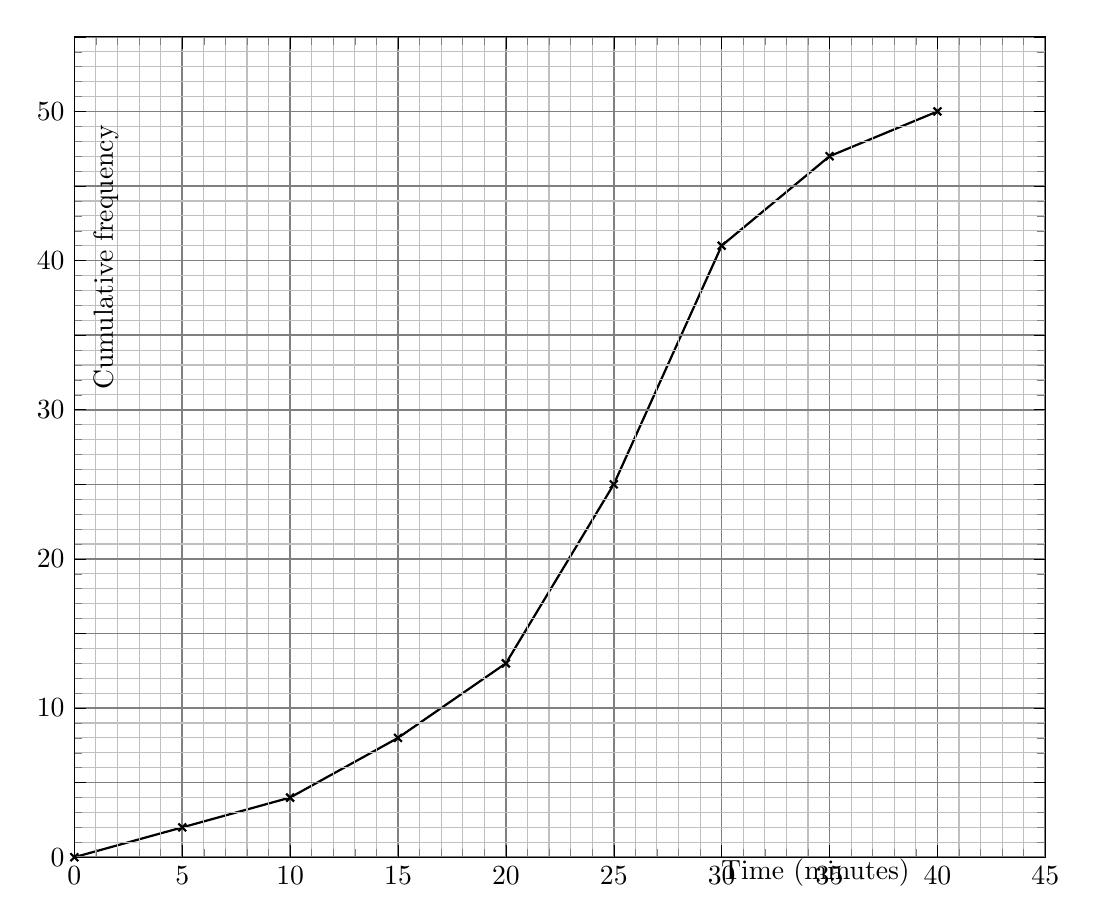
\begin{tikzpicture}
\centering

\begin{axis}[
area style,
height=12cm,
solid,
grid = both,
minor grid style=gray,
major grid style =black,
major grid style ={line width =0.6pt},
%	major grid style =thick,
major tick style=black,	
xmin = 0, xmax=45,
ymin=0, ymax= 55,
grid = both,
minor grid style=lightgray,
major grid style =gray,
major tick style=black,	
minor y tick num=4,
minor x tick num=4, 
xtick={0,5,10,15,20,25,30,35,40,45},
xticklabels={0,5,10,15,20,25,30,35,40,45},
ytick={0,5,10,15,20,25,30,35,40,45,50,55},
yticklabels={0,\empty,10,\empty,20,\empty,30,\empty,40,\empty,50,\empty},
x label style={at={(current axis.right of origin)},anchor=north, below=2mm, left =16mm},
y label style={at={(current axis.above origin)},anchor = west, below =4mm,left = 10mm},
xlabel={Time (minutes)},
ylabel={Cumulative frequency}
]	
\addplot[thick, solid,mark=x] plot coordinates { 
	(0,0)		
	(5,2)
	(10,4)
	(15,8)
	(20,13)
	(25,25)
	(30,41)
	(35,47)
	(40,50)		
};	
\end{axis}
\end{tikzpicture}

\medskip

 Use the graph to estimate
 
 \begin{enumerate}
 	\item how many people spent at least $17$ minutes but less than 27 minutes in the supermarket,
 	\item the value of $t$, where $60\%$ of the people spent less than $t$ minutes in the supermarket,
 	\item the value of $s$, where $60\%$ of the people spent at least $s$ minutes in the supermarket,
 	\item the median time,
 	\item the interquartile range.
 \end{enumerate}


\item  A factory produces certain components. In a quality control test, $500$ components were weighted and their weights recorded to the nearest gram. The table shows the results.

\medskip

\renewcommand{\arraystretch}{1.2} % default is 1.0
\begin{tabular}{|l|c|c|c|c|c|}
	\hline
	Weight (\si{\gram})  & $60-69$ & $70-74$ & $75-79$ & $80-84$ & $85-89$   \\ 
	\hline
	Frequency & $30$ & $90$ & $130$ & $210$ & $40$  \\ 
	\hline
\end{tabular}

\smallskip

\begin{enumerate}
	\item Construct a cumulative frequency table and draw a cumulative frequency graph.
	\item  Components that weight less than $64.5$ grams or more than $87.5$ grams were rejected. Use your graph to estimate the percentage of components that were accepted.
\end{enumerate}



\item  The cumulative frequency table shows the times taken by students to travel to college on a particular day.

\medskip

\renewcommand{\arraystretch}{1.2} % default is 1.0
\begin{tabular}{|l|c|c|c|c|c|}
	\hline
	Time (minutes)  & $ < 10 $ & $ < 15 $ & $ < 20 $ & $ <30 $ & $ <45 $   \\ 
	\hline
	Cumulative frequency & $35$ & $79$ & $157$ & $350$ & $400$  \\ 
	\hline
\end{tabular}

\smallskip

Construct a frequency table and use it to estimate the mean time taken 	to travel to college on that day.


\item The cumulative frequency table gives 	the heights of $400$ children in a certain school.

\medskip

\renewcommand{\arraystretch}{1.2} % default is 1.0
\begin{tabular}{|l|c|c|c|c|c|c|c|c|}
	\hline
	Height, $x$ \si{\cm}  & $ < 100 $ & $ < 110 $ & $ < 120 $ & $ <130 $ & $ <140 $ & $< 150$& $<160$& $<170$   \\ 
	\hline
	Cumulative frequency & $0$ & $27$ & $85$ & $215$ & $320$ & $370$ & $395$ & $400$  \\ 
	\hline
\end{tabular}

\smallskip

\begin{enumerate}
	\item Draw a cumulative frequency curve.
	\item Use the curve to estimate the median height
	\item Determine the interquatile range.
\end{enumerate}

\item The arrival times of $204$ trains were noted and the number of minutes, $t$, that each train was late was recorded.	

\medskip

\renewcommand{\arraystretch}{1.2} % default is 1.0
\begin{tabular}{|l|c|c|c|c|c|}
	\hline
	Number of minutes late ($t$)   & $ -2\leqslant t < 0 $ & $ 0\leqslant t < 2 $ & $ 2\leqslant t < 4 $ & $4\leqslant t < 6 $ & $ 6\leqslant t < 10 $   \\ 
	\hline
	Number of trains & $43$ & $51$ & $69$ & $22$ & $19$  \\ 
	\hline
\end{tabular}

\smallskip

\begin{enumerate}
	\item Explain what $-2\leqslant t <0$ means about the arrival times of the trains.
	\item Draw a cumulative frequency graph, and from it estimate the median and interquartile range of the number of minutes late of these trains.
\end{enumerate}


\item The times, to the nearest minute, taken by $120$ students to write a timed essay were recorded. The results are shown in the table.
 
 \medskip
 
 \renewcommand{\arraystretch}{1.2} % default is 1.0
 \begin{tabular}{|l|c|c|c|c|c|}
 	\hline
 	Time (minutes) ($t$)   & $ 40-44 $ & $ 45-49 $ & $ 50-54 $ & $ 55-59 $ & $ 60-64 $   \\ 
 	\hline
 	Frequency & $8$ & $24$ & $32$ & $30$ & $26$  \\ 
 	\hline
 \end{tabular}
 
 \smallskip
 
 \begin{enumerate}
 	\item Construct the cumulative frequency table and draw a cumulative frequency graph.
 	\item Use your graph to estimate the lower quartile and the median.
 \end{enumerate}

Another group of $40$ students wrote the same essay and all of them took at least 1 hour to complete it.

\begin{enumerate}
	\item Use your graph to estimate the lower quartile of all $160$ students.
	\item Explain why it is not possible to estimate the interquartile range of the times spent by all 160 students.
\end{enumerate}

\end{enumerate}


\newpage

%%%%%%%%%%%%%%%%%%%%%%%%%%%%%%%%%%%%%%%%%%%%%
%%%%%%%%%%%%%%%%%%%%%%%%%%%%%%%%%%%%%%%%%%%%%
%%%%%%%%%%%%%%%%%%%%%%%%%%%%%%%%%%%%%%%%%%%%%
%%%%%%%%%%%%%%%%%%%%%%%%%%%%%%%%%%%%%%%%%%%%%
%% 1.7 Box-and-whisker plot %%%
%%%%%%%%%%%%%%%%%%%%%%%%%%%%%%%%%%%%%%%%%%%%%
%%%%%%%%%%%%%%%%%%%%%%%%%%%%%%%%%%%%%%%%%%%%%
%%%%%%%%%%%%%%%%%%%%%%%%%%%%%%%%%%%%%%%%%%%%%
%%%%%%%%%%%%%%%%%%%%%%%%%%%%%%%%%%%%%%%%%%%%%
\subsection{Box-and-whisker plots}

In a box-and-whisker plot the median and quartiles are shown, as well as the $\underline{\hspace{2 cm}}$ and $\underline{\hspace{2 cm}}$ values of a distribution.

\medskip

For example, 	a survey on the heights of all the girls in a particular year group 	in a school gave the following information.

\begin{tabular}{lc}
	Minimum height  & 144 cm  \\
	Lower quartile~ & 159 cm  \\
	Median~         & 165 cm  \\
	Upper quartile~ & 169 cm  \\
	Maximum height  & 181 cm 
\end{tabular}

A box-and-whisker plot can be drawn as following:

\bigskip
\begin{figure}[!htpb]
\centering
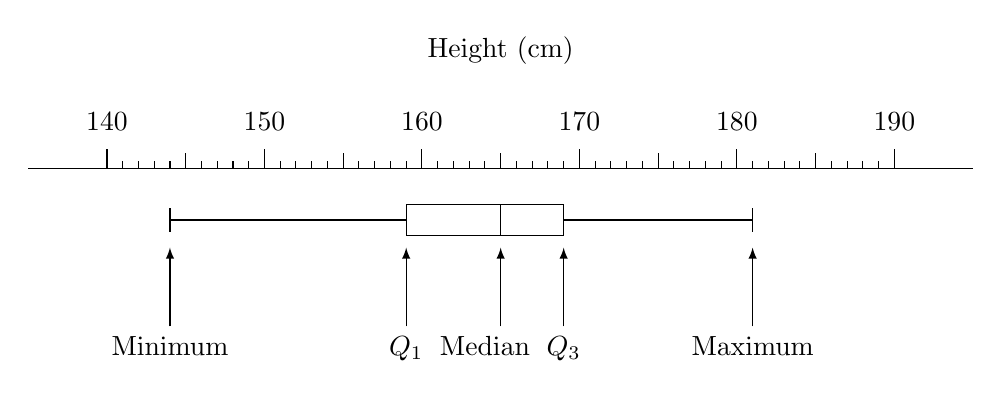
\begin{tikzpicture}

%\def\labelz{{"Judicial Independence","Long Label 2","Label 3","Label 4","180","190"}}
\draw [] (1,0) -- (13,0);
\foreach \x in {1,...,50} {%
	\draw [] (2+0.2*\x,0) -- (2+0.2*\x,0.1);
	
}
\foreach \x in {1,...,10} {%
	\draw [] (2+\x,0) -- (2+\x,0.2);
	
}
\foreach \x in {1,...,6} {%
	\draw [] (2*\x,0) -- (2*\x,0.25);
	\node at (2*\x,0.6){\pgfmathparse{int(130+10*\x)}\pgfmathresult};
}


\draw  (2.8,-0.8) -- (2.8, -0.5);

\draw  (2.8, -0.65) -- (5.8, -0.65);

\draw (5.8,-0.85) rectangle (7.8,-0.45);

\draw (7.8,-0.65) -- (10.2,-0.65);

\draw (10.2,-0.8) -- (10.2,-0.5);

\draw (7,-0.45) -- (7,-0.85);



\draw[-latex] (2.8, -2) -- (2.8,-1) node[below,yshift=-1cm]{Minimum}; 
\draw[-latex] (5.8, -2) -- (5.8,-1) node[below,yshift=-1cm]{ $Q_1$}; 
\draw[-latex] (7, -2) -- (7,-1) node[below,yshift=-1cm,xshift=-0.2cm]{Median}; 
\draw[-latex] (7.8, -2) -- (7.8,-1) node[below,yshift=-1cm]{ $Q_3$}; 
\draw[-latex] (10.2, -2) -- (10.2,-1) node[below,yshift=-1cm]{Maximum}; 

\draw (7,1.5) node{Height (cm)};




\end{tikzpicture} 
\caption{Box-and-whisker plot to show heights of $15$-year-old girl  }

\end{figure}

Tips on drawing the box-and-whisker plot:

\begin{itemize}
	\setlength\itemsep{0.8em}
	\item The scale must be $\underline{\hspace{2 cm}}$ and $\underline{\hspace{2 cm}}$.
	\item The whiskers must not be drawn through the box.
	
\end{itemize}

The shape of a distribution:

\medskip
\vspace{3cm}

Positive skew  \hspace{4.2cm} Symmetrical  \hspace{4.2cm} \hfill Negative skew

\exercise  %%% --  Exercise 8 

\begin{enumerate}
	\item Two groups of people played a computer game which tested  how quickly they reacted to a  visual instruction to press a particular key. The computer measured reaction times in seconds, to the nearest tenth of a second. The following summary statistics were displayed for each group.
	
	\begin{table}[!htpb]
		\centering
		\begin{tabular}{|l|c|c|c|c|c|} 
			\cline{2-6}
			\multicolumn{1}{l|}{} & Minimum & Lower quartile, Q1 & Median, Q2 & Upper quartile, Q3 & Maximum  \\ 
			\hline
			Group 1               & 0.6     & 0.8                & 1.0        & 1.5                & 1.9      \\ 
			\hline
			Group 2               & 0.4     & 0.7                & 1.0        & 1.3                & 1.6      \\
			\hline
		\end{tabular}
	\end{table}

Draw two box-and-whisker plots and compare the reaction time of the two groups.


   \item The following back-to-back stem-and-leaf diagram show the cholesterol count for a group of $45$ people who exercise daily and for another group of $63$ who do not exercise. The figures in brackets show the number of people corresponding to each set of leaves.
  \setlength{\tabcolsep}{1mm}  %% set column width of a table
   \begin{table}[!htpb]
   	\centering
   	\begin{tabular}{lllllllllllll|c|lllllllllllllll}
   		\multicolumn{13}{c}{People who exercise}             & \multicolumn{1}{c}{} & \multicolumn{15}{l}{People who do not exercise}               \\
   		(9)  &   &   &   & 9 & 8 & 7 & 6 & 4 & 3 & 2 & 2 & 1 & 3                    & 1 & 5 & 7 & 7 &   &   &   &   &   &   &   &   &   &   & (4)   \\
   		(12) & 9 & 8 & 8 & 8 & 7 & 6 & 6 & 5 & 3 & 3 & 2 & 2 & 4                    & 2 & 3 & 4 & 4 & 5 & 8 &   &   &   &   &   &   &   &   & (6)   \\
   		(9)  &   &   &   & 8 & 7 & 7 & 7 & 6 & 5 & 3 & 3 & 1 & 5                    & 1 & 2 & 2 & 2 & 3 & 4 & 4 & 5 & 6 & 7 & 8 & 8 & 9 &   & (13)  \\
   		(7)  &   &   &   &   &   & 6 & 6 & 6 & 6 & 4 & 3 & 2 & 6                    & 1 & 2 & 3 & 3 & 3 & 4 & 5 & 5 & 5 & 7 & 7 & 8 & 9 & 9 & (14)  \\
   		(3)  &   &   &   &   &   &   &   &   &   & 8 & 4 & 1 & 7                    & 2 & 4 & 5 & 5 & 6 & 6 & 7 & 8 & 8 &   &   &   &   &   & (9)   \\
   		(4)  &   &   &   &   &   &   &   &   & 9 & 5 & 5 & 2 & 8                    & 1 & 3 & 3 & 4 & 6 & 7 & 9 & 9 & 9 &   &   &   &   &   & (9)   \\
   		(1)  &   &   &   &   &   &   &   &   &   &   &   & 4 & 9                    & 1 & 4 & 5 & 5 & 8 &   &   &   &   &   &   &   &   &   & (5)   \\
   		(0)  &   &   &   &   &   &   &   &   &   &   &   &   & 10                   & 3 & 3 & 6 &   &   &   &   &   &   &   &   &   &   &   & (3)  
   	\end{tabular}
   
    \vspace{4 pt}
   
    
    \fbox{\parbox{3.5in}{Key:  $2 |8|1$ represents a cholesterol count  of 8.2  in the group who exercise 
    		and 8.1 in the group who do not exercise}}
    
  
   \end{table}
	
	
	\begin{enumerate}
		\item Give one useful feature of a stem-and-leaf diagram.
		\item Find the median and quartiles of the cholesterol count for the group who do not exercise.
		
		
	\end{enumerate}
	 
	 You are given that the lower quartile, median and upper quartile of the cholesterol  count for the group who exercise are $4.25$, $5.3$ and $6.6$ respectively.
	 \begin{enumerate}[resume ]
	 	\item On a single diagram on graph, draw two box-and-whisker plots to illustrate the data.
	 \end{enumerate}
 
 \item  The cumulative frequency graph below shows the marks of two groups of 120 people in a test.
 
 \medskip
 
 
 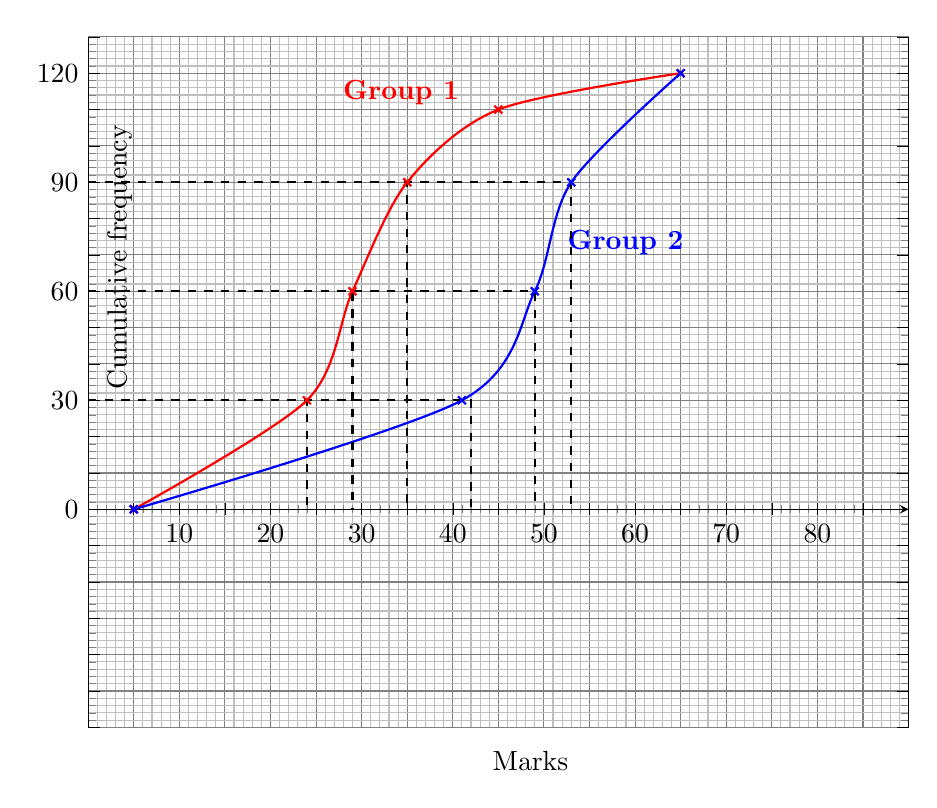
\begin{tikzpicture}
 \centering
 
 \begin{axis}[
 width = 12cm,
 axis x line = middle,
 xmin = 0, xmax=90,
 ymin=-60, ymax= 130,
 grid = both,
 minor grid style=lightgray,
 ytick={-60,-50,-40,-30,-20,-10,0,10,20,30,
 	40,50,60,70,80,90,100,110,120,130},
 yticklabels={\empty,\empty,\empty,\empty,\empty,\empty,0,\empty,\empty,30,
 	          \empty,\empty,60,\empty,\empty,90,\empty,\empty,120,\empty
         },
 xtick={0,5,10,15,20,25,30,35,40,45,50,55,60,65,70,75,80,85,90},
 xticklabels={0,\empty,10,\empty,20,\empty,30,\empty,40,\empty,50,\empty,60,\empty,70,\empty,80,\empty,\empty},
 major grid style =gray,
 major tick style=black,	
 minor x tick num=4,
 minor y tick num=4, 
 %extra x ticks={5,15,25,35,45,},
 %extra x tick labels={5,15,25,35,45},
 %extra y ticks={5,15,25,35,45,55},
 %extra y tick labels={\empty,\empty,\empty,\empty,\empty},
 %extra tick style={
 %	tick style=thick
 %},	
 %yticklabels={\empty,\empty,\empty},
 x label style={at={(current axis.right of origin)},anchor=north, below=3.2cm, left =4.2cm},
 y label style={at={(current axis.above origin)},anchor = west, below =4mm,left = 10mm},
 xlabel={Marks},
 ylabel={Cumulative frequency}
 ]	
 \addplot[thick, mark=x,smooth,red] plot coordinates { 
 	(5,0)		
 	(24,30)
 	(29,60)
 	(35,90)
 	(45,110)
 	(65,120)		
 } node[xshift=-3.55cm,yshift=-0.25cm]{\textbf{Group 1}};	
\addplot[thick, mark=x,smooth,blue] plot coordinates { 
	(5,0)		
	(41,30)
	(49,60)
	(53,90)
	(65,120)		
}node[xshift=-0.7cm,yshift=-2.15cm]{\textbf{Group 2}};	

\addplot[dashed,thick] plot coordinates {
 (0,30)
 (24,30)
 (24,0)
 
};
\addplot[dashed,thick] plot coordinates {
	(0,60)
	(29,60)
	(29,0)
	
};
\addplot[dashed,thick] plot coordinates {
	(0,90)
	(35,90)
	(35,0)
	
};

\addplot[dashed,thick] plot coordinates {
	(0,30)
	(42,30)
	(42,0)
	
};
\addplot[dashed,thick] plot coordinates {
	(0,60)
	(49,60)
	(49,0)
	
};
\addplot[dashed,thick] plot coordinates {
	(0,90)
	(53,90)
	(53,0) 
	
};
 \end{axis}
 \end{tikzpicture}
 
 \medskip
 
 
 Draw two box-and-whisker plots for each group on the same diagram, and compare the two sets of data, state why it is misleading by the cumulative frequency curves.
 
 
	
\end{enumerate}

\newpage 

\subsection{Choosing measures and diagrams}
When representing data  you need to  consider the ways that would be most  appropriate,

\begin{itemize}
\setlength\itemsep{1.8em}
	\item What type of diagram should you draw?
	\item  Which average best represent the data?
	\item Which measure of spread is most informative?
\end{itemize}

\vspace{2cm}
Measure of central tendency:

\begin{table}[!htpb]
	\begin{tabular}{|l|p{6.5cm}|p{6.5cm}|}
		\hline
		& \textbf{Advantages} & \textbf{Disadvantages} \\ \hline
		Mode   &  It is useful when the post popular category is needed.          &  Very small data or more than two modes.
		
			 There may not be a mode.
			 
		 Not representative.
		 
			 The modal class depends on the grouping of data.
	           \\ \hline
		Median &     It is not affected by extreme values.       &   Not use the information of the whole data set            \\ \hline
		Mean   &      Use all the data and so represent every item      &    It is affected by one or two extreme values           \\ \hline
	\end{tabular}
\end{table}

\vspace{2cm}

Measure of spread:

\begin{table}[!htpb]
	\begin{tabular}{|l|p{5.5cm}|p{6cm}|}
		\hline
		& \textbf{Advantages} & \textbf{Disadvantages} \\ \hline
		Range   &  Easy to calculate. 
		
		Represent the complete spread of data.
		         &  It can be affected by extreme values.
		\\ \hline
		Interquartile range &     It is not affected by extreme values.       &   It depends only on particular values when the data was ranked.            \\ \hline
		Standard deviation   &      Use all the data and so represent every item.  
		
		It is useful in comparing two sets of data, to show the consistence.
		    &    It is affected by one or two extreme values.           \\ \hline
	\end{tabular}
\end{table}

\newpage 
Diagrams:

\begin{table}[!htpb]
	\begin{tabular}{|l|p{5cm}|p{5cm}|}
		\hline
		& \textbf{Advantages} & \textbf{Disadvantages} \\ \hline
		
		
		Stem-and-leaf diagram   &  It shows all the original data.
		
		It shows the shape of the distribution.
		
		The mode, median and quartile can be found.
		
		It is useful for comparing two sets of data.
	
		&  It is not suitable for large amount of data.
		\\ \hline
		
		
		Histogram &     It can represent groups of different widths.
		
		It shows whether the distribution is symmetrical or skew
		
		The mean and the standard deviation can be estimated from the histogram.       &   The visual impact can be altered by choosing different groups.
		
		Two distributions cannot be shown on the same diagram.           \\ \hline
		
		
		Cumulative frequency graph   &      The median and quartiles can be estimated the graph.  
		
		Sets of data can be compared by drawing graphs on the same diagram
		&    The visual impact can be altered by using different scales.           \\ \hline
		
		Box-and-whisker plot   &      It is easy to see whether the distribution is symmetrical or whether  there is a tail to the left or right.
		
		It can be used to find the extreme values.
		
		It is easy to see the range and interquartile range.
		
		You can compare two or more sets of data by drawing plots on the same diagram.
		&    It does not show frequencies.           \\ \hline
	\end{tabular}
\end{table}


\newpage

%%%%%%%%% 
%%%%%%%%%
%%%   %%%%%
%%%  Miscelaneous 1
%%%%%%%
%%%%%%%%
%%%%%%%%%%
%%%%%%%%%

\mis

\begin{enumerate}
	
	\item  A company manager, faced with the possibility of having to reduce staff during a recsssion, compiles a table of the ages of his employees.
	
	 \medskip
	
	\renewcommand{\arraystretch}{1.2} % default is 1.0
	\begin{tabular}{|l|c|c|c|c|c|c|}
		\hline
		Age, completed years   & $ 20-30 $ & $ 31-35 $ & $ 36-40 $ & $ 41-45 $ & $ 46-50 $  & $51-60$  \\ 
		\hline
		Number in age group & $5$ & $7$ & $18$ & $30$ & $16$ & $9$ \\ 
		\hline
	\end{tabular}

   \medskip
   
   Draw:
   \begin{enumerate}
   	\item a cumulative frequency graph and so find estimates for the three quartiles,
   	\item a histogram,
   	\item a box-and-whisker plot,
   \end{enumerate}
   to illustreate these figures.
	
	



   \item   The monthly salaries, $w$ dollars, of $10$ women are such that $\displaystyle \sum (w-300) = -200$. 

The monthly salaries, $m$ dollars, of $20$ men are such that $\displaystyle \sum (m-4000) =120$.

\begin{enumerate}
	\item Find the difference between the mean monthly salary of the women and the mean monthly salary of the men.
	\item Find the mean monthly salary of all the women and men together.
\end{enumerate}


\item Eighty candidates took an examination in Astronomy, for which no candidate scored more than $80\%$. The examiners suggest that five grades, $A$, $B$, $C$, $D$ and $E$, should be awarded to these candidates, using upper grade boundaries $64$, $50$, $36$ and $26$ for grades $B$, $C$, $D$ and $E$, respectively. In this case, grades $A$, $B$, $C$, $D$ and $E$, will be awarded in the ratio $1:3:5:4:3$.

\begin{enumerate}
	\item Using the examiners' suggestion, represent the scores in a cumulative frequency graph and use it to estimate the median score.
	\item All of the grade boundaries are later reduced by $10\%$. Estimate how many candidates will be awarded a higher grade because of this.
\end{enumerate}

\item A set of $n$ pieces of data has mean $\bar{x}$ and standard deviation $S$. Another set of $2n$ pieces of data has mean $\bar{x}$ and standard deviation $\frac{1}{2}S$. Find the standard deviation of all these pieces of data together in term of $S$.

\item The daily journey times for $80$ bank staff to get to work are given in the following table.

	 \medskip

\renewcommand{\arraystretch}{1.2} % default is 1.0
\begin{tabular}{|l|c|c|c|c|c|c|c|}
	\hline
	Time ($t$ min)  & $ t<10 $ & $ t<15 $ & $ t<20 $ & $ t<25$ & $ t<30 $  & $t<45$ & $t<60$  \\ 
	\hline
	No.staff (cf) & $3$ & $11$ & $24$ & $56$ & $68$ & $76$  &  $80$ \\ 
	\hline
\end{tabular}

\medskip

\begin{enumerate}
	\item How many staff take between $15$  and $45$ minutes to get to work?
	\item Find the exact number of staff who take $\frac{x+y}{2}$ minutes or more to get to work, given that $85\%$ of the staff take less than $x$ minutes and that $70\%$ of the staff take $y$ minutes or more.
\end{enumerate}



\end{enumerate}










\newpage 
\exam

\begin{enumerate}
	%%%%%%%%%%%%%%%%%%%%%%%%%%%%%%%%%%%%%
	%%%%%%%%%%%%%%%%%%%%%%%%%%%%%%%%%%%%%
	%%%%%%%%%%%%%%%%%%%%%%%%%%%%%%%%%%%%%
	%%% Question 1  9709 s16 qp62  Q2 %%%%
	%%%%%%%%%%%%%%%%%%%%%%%%%%%%%%%%%%%%%
	%%%%%%%%%%%%%%%%%%%%%%%%%%%%%%%%%%%%%
	%%%%%%%%%%%%%%%%%%%%%%%%%%%%%%%%%%%%%
	\item Anabel measured the lengths, in centimetres, of $200$ caterpillars. Her results are illustrated in the	cumulative frequency graph below.
	
	 \medskip
	
	
	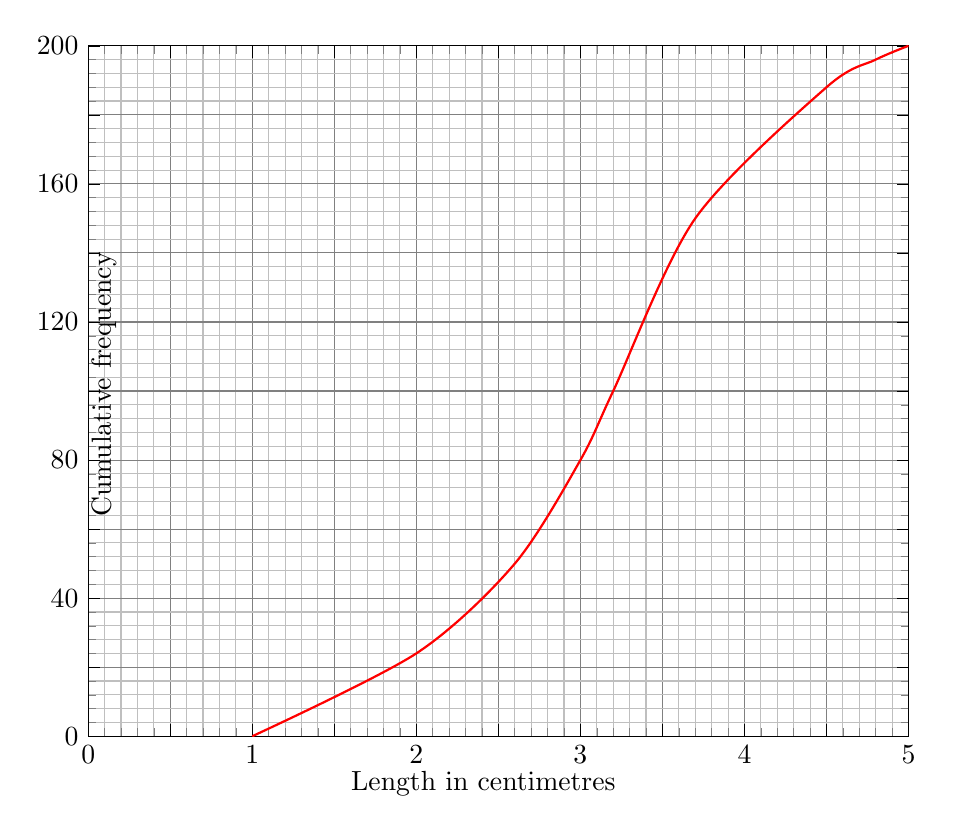
\begin{tikzpicture}
		\centering
		
		\begin{axis}[
			width = 12cm,
			%axis x line = middle,
			xmin = 0, xmax=5,
			ymin=0, ymax= 200,
			grid = both,
			minor grid style=lightgray,
			ytick={0,20,40,60,80,
				100,120,140,160,180,
				200},
			yticklabels={0,\empty,40,\empty,80,
				\empty,120,\empty,160,\empty,
				200
			},
			xtick={0,0.5,1,1.5,2,
				2.5,3,3.5,4,4.5,
				5},
			xticklabels={0,\empty,1,\empty,2,
			\empty,3,\empty,4,\empty,
			5},
			major grid style =gray,
			major tick style=black,	
			minor x tick num=4,
			minor y tick num=4, 
			%extra x ticks={5,15,25,35,45,},
			%extra x tick labels={5,15,25,35,45},
			%extra y ticks={5,15,25,35,45,55},
			%extra y tick labels={\empty,\empty,\empty,\empty,\empty},
			%extra tick style={
			%	tick style=thick
			%},	
			%yticklabels={\empty,\empty,\empty},
			x label style={at={(current axis.right of origin)},anchor=north, below=0.6cm, left =3.6cm},
			y label style={at={(current axis.above origin)},anchor = west, below =2mm,left = 25mm},
			xlabel={Length in centimetres},
			ylabel={Cumulative frequency}
			]	
			\addplot[thick, mark=none,smooth,red] plot coordinates { 
				(1,0)
				(2,24)
				(2.6,50)		
				(3,80)
				(3.2,100)
				(3.7,150)
				(4.5,188)
				(4.8,196)
				(5,200)
						
			} ;	
			
		\end{axis}
	\end{tikzpicture}
	
	\medskip
	
	\begin{enumerate}[label=(\roman*)]
		\item Estimate the median and the interquartile range of the lengths. \hfill [3]
		\item Estimate how many caterpillars had a length of between $2$ and $3.5$ \si{\cm}. \hfill [1]
		\item $6\%$ of caterpillars were of length $l$ centimetres or more. Estimate $l$. \hfill [2]
	\end{enumerate}

%%%%%%%%%%%%%%%%%%%%%%%%%%%%%%%%%%%%%
%%%%%%%%%%%%%%%%%%%%%%%%%%%%%%%%%%%%%
%%%%%%%%%%%%%%%%%%%%%%%%%%%%%%%%%%%%%
%%% Question 2  9709 w18 qp63  Q7 %%%%
%%%%%%%%%%%%%%%%%%%%%%%%%%%%%%%%%%%%%
%%%%%%%%%%%%%%%%%%%%%%%%%%%%%%%%%%%%%
%%%%%%%%%%%%%%%%%%%%%%%%%%%%%%%%%%%%%

\item 



 The heights, in \si{\cm}, of the $11$ members of the Anvils athletics team and the $11$ members of the Brecons swimming team are shown below.
 
 	 \medskip
 
 \renewcommand{\arraystretch}{1.2} % default is 1.0
 \begin{tabular}{|l|c|c|c|c|c|c|c|c|c|c|c|}
 	\hline
 	Anvils  & $ 173 $ & $ 158 $ & $ 180 $ & $ 196$ & $175 $  & $165$ & $170$ & $169$& $181$& $184$ & $172$ \\ 
 	\hline
 	Brecons & $ 166 $ & $ 170 $ & $ 171 $ & $ 172$ & $172 $  & $178$ & $181$ & $182$& $183$& $183$ & $192$ \\ 
 	\hline
 \end{tabular}
 
 \medskip
 
 \begin{enumerate}[label=(\roman*)]
 	\item Draw a back-to-back stem-and-leaf diagram to represent this information, with Anvils on the
 	left-hand side of the diagram and Brecons on the right-hand side. \hfill [4]
 	
 	\item Find the median and the interquartile range for the heights of the Anvils. \hfill [3]
 \end{enumerate}

The heights of the $11$ members of the Anvils are denoted by $x$ \si{\cm}. It is given that $ \sum x =1923$, and  $\sum x^2 =337 221$. Suppose the Anvils are joined by $3$ new members whose heights are $166$ \si{\cm}, $172$ \si{\cm} and $182$ \si{\cm}.

\begin{enumerate}[resume,label=(\roman*)]
	\item Find the standard deviation of the heights of all $14$ members of the Anvils.\hfill  [4]
\end{enumerate}


%%%%%%%%%%%%%%%%%%%%%%%%%%%%%%%%%%%%%
%%%%%%%%%%%%%%%%%%%%%%%%%%%%%%%%%%%%%
%%%%%%%%%%%%%%%%%%%%%%%%%%%%%%%%%%%%%
%%% Question 3  9709 w19 qp62  Q3 %%%%
%%%%%%%%%%%%%%%%%%%%%%%%%%%%%%%%%%%%%
%%%%%%%%%%%%%%%%%%%%%%%%%%%%%%%%%%%%%
%%%%%%%%%%%%%%%%%%%%%%%%%%%%%%%%%%%%%

\item  The speeds, in \si{\km\per\hour}, of $90$ cars as they passed a certain marker on a road were recorded, correct to the nearest \si{\km\per\hour}. The results are summarised in the following table.


\medskip

\renewcommand{\arraystretch}{1.2} % default is 1.0
\begin{tabular}{|l|c|c|c|c|c|}
	\hline
	Speeds (\si{\km\per\hour})  & $ 10-29 $ & $ 30-39 $ & $ 40-49 $ & $ 50-59$ & $60-89$ \\ 
	\hline
	Frequency & $ 10$ & $ 24 $ & $ 30$ & $ 14$ & $12 $ \\ 
	\hline
\end{tabular}

\medskip

\begin{enumerate}[label=(\roman*)]
	\item On the grid, draw a histogram to illustrate the data in the table. \hfill [4]
	\item Calculate an estimate for the mean speed of these $90$ cars as they pass the marker. \hfill [2]
\end{enumerate}


%%%%%%%%%%%%%%%%%%%%%%%%%%%%%%%%%%%%%
%%%%%%%%%%%%%%%%%%%%%%%%%%%%%%%%%%%%%
%%%%%%%%%%%%%%%%%%%%%%%%%%%%%%%%%%%%%
%%% Question 4  9709 s18 qp63  Q4 %%%%
%%%%%%%%%%%%%%%%%%%%%%%%%%%%%%%%%%%%%
%%%%%%%%%%%%%%%%%%%%%%%%%%%%%%%%%%%%%
%%%%%%%%%%%%%%%%%%%%%%%%%%%%%%%%%%%%%

\item  Farfield Travel and Lacket Travel are two travel companies which arrange tours abroad. The numbers
of holidays arranged in a certain week are recorded in the table below, together with the means and
standard deviations of the prices.

\medskip

\begin{table}[!htpb]
	\centering
	\renewcommand{\arraystretch}{1.2} % default is 1.0
	\begin{tabular}{l|c|c|c|}
		\cline{2-4}
		& Number of holidays & Mean price ($\$$) & Standard deviation ($\$$) \\ \hline
		\multicolumn{1}{|l|}{Farfield Travel} & $30$                 & $1500$            & $230 $                    \\ \hline
		\multicolumn{1}{|l|}{Lacket Travel}   & $21$                 & $2400 $           & $160  $                   \\ \hline
	\end{tabular}
\end{table}

\medskip

\begin{enumerate}[label=(\roman*)]
	\item Calculate the mean price of all $51$ holidays. \hfill [2]
	\item The prices of individual holidays with Farfield Travel are denoted by $\$ x_F$	and the prices of
	individual holidays with Lacket Travel are denoted by $\$x_L$. By first finding $\sum x_F^2$ and  $\sum x_L^2$, find the standard deviation of the prices of all $51$ holidays. \hfill[5]
\end{enumerate}


%%%%%%%%%%%%%%%%%%%%%%%%%%%%%%%%%%%%%
%%%%%%%%%%%%%%%%%%%%%%%%%%%%%%%%%%%%%
%%%%%%%%%%%%%%%%%%%%%%%%%%%%%%%%%%%%%
%%% Question 5  9709 s19 qp61  Q4 %%%%
%%%%%%%%%%%%%%%%%%%%%%%%%%%%%%%%%%%%%
%%%%%%%%%%%%%%%%%%%%%%%%%%%%%%%%%%%%%
%%%%%%%%%%%%%%%%%%%%%%%%%%%%%%%%%%%%%

\item The Mathematics and English A-level marks of $1400$ pupils all taking the same examinations are
shown in the cumulative frequency graphs below. Both examinations are marked out of $100$.

\medskip


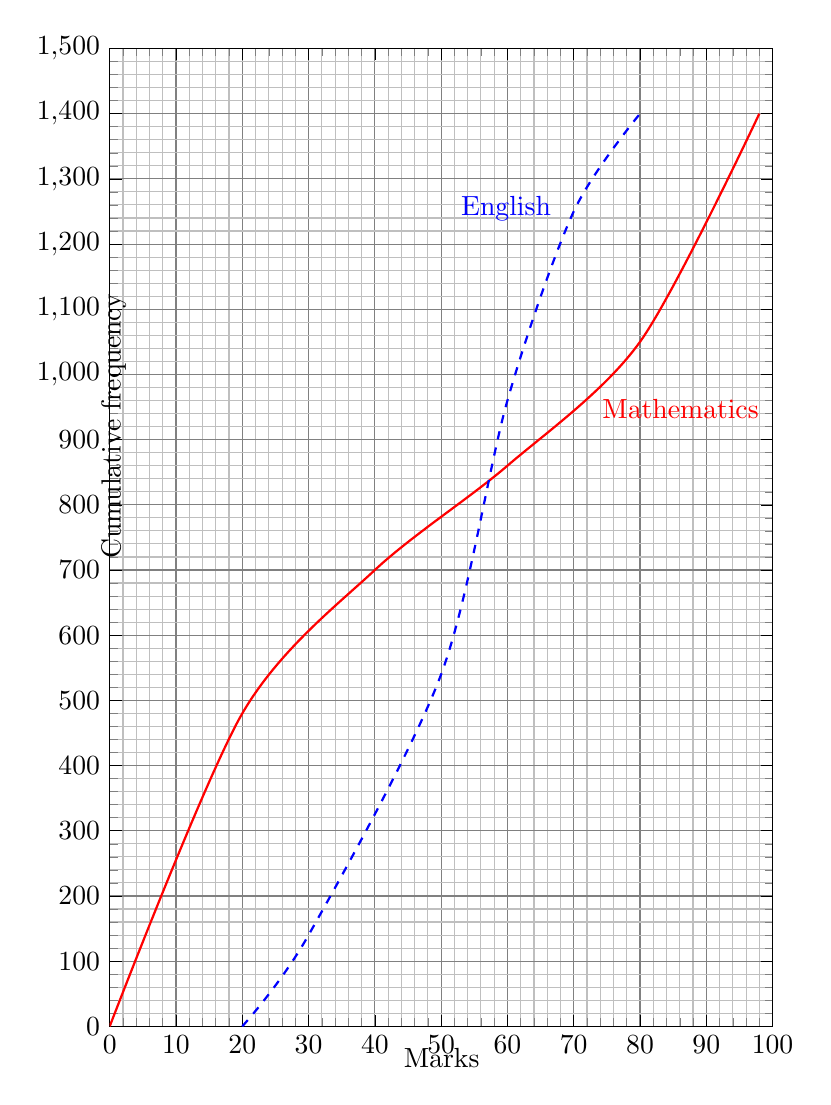
\begin{tikzpicture}
	\centering
	
	\begin{axis}[
		width = 10cm,
		height = 14cm,
		%axis x line = middle,
		xmin = 0, xmax=100,
		ymin=0, ymax= 1500,
		grid = both,
		minor grid style=lightgray,
		ytick={0,100,200,300,400,
			500,600,700,800,900,
			1000,1100,1200,1300,1400,1500},
	%	yticklabels={0,\empty,40,\empty,80,
	%		\empty,120,\empty,160,\empty,
	%		200
	%	},
		xtick={0,10,20,30,40,50,
			60,70,80,90,100},
	%	xticklabels={0,\empty,1,\empty,2,
	%		\empty,3,\empty,4,\empty,
	%		5},
		major grid style =gray,
		major tick style=black,	
		minor x tick num=4,
		minor y tick num=4, 
		%extra x ticks={5,15,25,35,45,},
		%extra x tick labels={5,15,25,35,45},
		%extra y ticks={5,15,25,35,45,55},
		%extra y tick labels={\empty,\empty,\empty,\empty,\empty},
		%extra tick style={
		%	tick style=thick
		%},	
		%yticklabels={\empty,\empty,\empty},
		x label style={at={(current axis.right of origin)},anchor=north, below=0.4cm, left =3.6cm},
		y label style={at={(current axis.above origin)},anchor = west, below =0.5mm,left = 30mm},
		xlabel={Marks},
		ylabel={Cumulative frequency}
		]	
		\addplot[thick, mark=none,smooth,red] plot coordinates { 
			(0,0)
		%	(2,100)
			(20,480)
		%	(30,600)
			(40,700)
			(60,860)
			(80,1050)
			(98,1400)			
		} node[below,yshift=-3.5cm,xshift=-1cm]{Mathematics};	
	\addplot[thick, mark=none,smooth,blue,dashed] plot coordinates { 
		(20,0)
		%	(2,100)
		(30,140)
		%	(30,600)
		(50,540)
		(60,960)
		(70,1250)
		(80,1400)			
	}node[left,xshift=-1.0cm,yshift=-1.2cm]{English} ;	
		
	\end{axis}
\end{tikzpicture}

Use suitable data from these graphs to compare the central tendency and spread of the marks in
Mathematics and English. \hfill [6]


%%%%%%%%%%%%%%%%%%%%%%%%%%%%%%%%%%%%%
%%%%%%%%%%%%%%%%%%%%%%%%%%%%%%%%%%%%%
%%%%%%%%%%%%%%%%%%%%%%%%%%%%%%%%%%%%%
%%% Question 6  9709 w18 qp62  Q2 %%%%
%%%%%%%%%%%%%%%%%%%%%%%%%%%%%%%%%%%%%
%%%%%%%%%%%%%%%%%%%%%%%%%%%%%%%%%%%%%
%%%%%%%%%%%%%%%%%%%%%%%%%%%%%%%%%%%%%

\item The following back-to-back stem-and-leaf diagram shows the reaction times in seconds in an
experiment involving two groups of people, $A$ and $B$.

\begin{table}[!htpb]
	\centering
	 \setlength{\tabcolsep}{2.2mm}  %% set column width of a table
	\begin{tabular}{cllllllll|l|cllllllll}
		\multicolumn{9}{c|}{$A$}              &    & \multicolumn{9}{c}{$B$}               \\ \hline
		(4) &   &   &   &   & 4 & 2 & 0 & 0 & 20 & 5 & 6 & 7 &   &   &   &   &   & (3) \\
		(5) &   &   &   & 9 & 8 & 5 & 0 & 0 & 21 & 1 & 2 & 2 & 3 & 7 & 7 &   &   & (6) \\
		(8) & 9 & 8 & 7 & 5 & 3 & 2 & 2 & 2 & 22 & 1 & 3 & 5 & 6 & 6 & 8 & 9 &   & (7) \\
		(6) &   &   & 8 & 6 & 7 & 5 & 2 & 1 & 23 & 4 & 5 & 7 & 8 & 8 & 9 & 9 & 9 & (8) \\
		(3) &   &   &   &   &   & 8 & 6 & 3 & 24 & 2 & 4 & 5 & 6 & 7 & 8 & 8 &   & (7) \\
		(1) &   &   &   &   &   &   &   & 0 & 25 & 0 & 2 & 7 & 8 &   &   &   &   & (4)
	\end{tabular}

 \vspace{4 pt}


\fbox{\parbox{4.8in}{Key:  $5 |22|6$ means a reaction time of $0.225$ seconds for $A$ and $0.226$ seconds for $B$}}
\end{table}

\begin{enumerate}[label=(\roman*)]
	\item Find the median and the interquartile range for group $A$. \hfill[3]

\end{enumerate}

The median value for group $B$ is $0.235$ seconds, the lower quartile is $0.217$ seconds and the upper
quartile is $0.245$ seconds.

\begin{enumerate}[resume,label=(\roman*)]
	\item Draw box-and-whisker plots for groups $A$ and $B$ on the grid. \hfill [3]
	
	
	\medskip
	\vspace{1cm}
	
	
	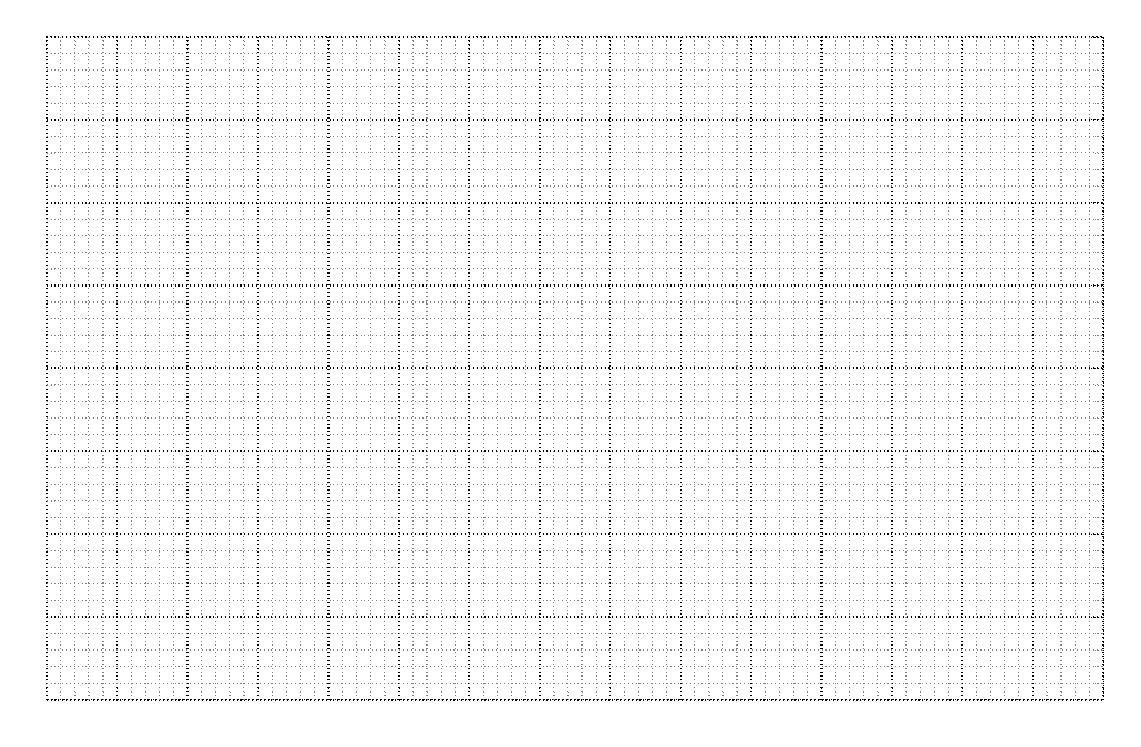
\begin{tikzpicture}
		\centering
		
		\begin{axis}[densely dotted,
			grid = both,
			minor grid style=gray,
			major grid style =black,
			major grid style ={line width =0.8pt},
			%	major grid style =thick,
			major tick style=black,	
			width = 15cm,	
			height = 10cm,		
			%axis x line = middle,
			xmin = 0, xmax=15,
			ymin=0, ymax= 8,			
			ytick={0,1,2,3,4,5,6,7,8},
			yticklabels={\empty,\empty,\empty,\empty,\empty,
				\empty,\empty,\empty,\empty
				},
			xtick={0,1,2,3,4,5,6,7,8,9,10,11,12,13,14,15},
			xticklabels={\empty,\empty,\empty,\empty,
				\empty,\empty,\empty,\empty,
				\empty,\empty,\empty,\empty,
				\empty,\empty,\empty,\empty
			},			
			minor x tick num=4,
			minor y tick num=4, 
			%extra x ticks={5,15,25,35,45,},
			%extra x tick labels={5,15,25,35,45},
			%extra y ticks={5,15,25,35,45,55},
			%extra y tick labels={\empty,\empty,\empty,\empty,\empty},
			%extra tick style={
			%	tick style=thick
			%},	
			%yticklabels={\empty,\empty,\empty},
			x label style={at={(current axis.right of origin)},anchor=north, below=0.4cm, left =3.6cm},
			y label style={at={(current axis.above origin)},anchor = west, below =0.5mm,left = 30mm},
			xlabel={},
			ylabel={}
			]	
		
					\end{axis}
	\end{tikzpicture}
\end{enumerate}







\end{enumerate}
















